\chapter{Revisão da Literatura}
\label{cap:02}
Neste capítulo, serão apontados os levantamentos bibliográficos realizados para esta pesquisa. Nele, serão apresentados os seguintes temas: dificuldades existentes na programação, linguagens de programação nativas e híbridas voltadas para desenvolvimento de dispositivos móveis, qualidade de código e trabalhos relacionados a este trabalho.

\section{Dificuldades Existentes na Programação}

Devido a rápida popularização dos aplicativos e sua fácil e prática utilização, os iniciantes podem acabar optando por entrar no ramo de desenvolvimento de \textit{software} com a ideia de conquistar uma vida financeira próspera por meio da disponibilização de uma aplicação simples em qualquer uma das famosas lojas disponíveis, e isso sem maiores esforços. No entanto, o aprendizado em tecnologia da informação, assim como em qualquer outra área/ramo, demanda empenho e prática. Um estudante de ciências contábeis, administração leva um tempo para se adaptar à normas e cálculos atuais, da mesma forma como um estudante da área da saúde não realiza manobras de salvamento sem conhecimento prévio, o mesmo conceito se aplica na programação.
Pular os fundamentos da área pode ser uma das piores práticas, pois o conhecimento básico aplica-se a todos os tipos de desenvolvimento, seja ele voltado para \textit{web}, \textit{desktop} ou \textit{mobile} \cite{Unipe2018}. 

O ato de desenvolver uma simples solução ou um \textit{software} extremamente complexo demanda muito mais do que apenas escrever um algoritmo em uma determinada linguagem e tecnologia.
O mais comum na área de tecnologia, é trabalhar e dar manutenção em um sistema que já está sendo utilizado, e que foi escrito por outros profissionais, para realizar qualquer modificação, faz-se necessário \textbf{compreender} toda a estrutura, conseguir visualizar/imaginar as consequências de cada futura alteração. Na maioria das vezes um código mais enxuto é sempre superior a outro com inúmeros trechos inúteis de códigos desnecessários. Nesse momento fazem-se úteis as melhorias internas como \textbf{reescrita} usando técnicas como \textit{TDD}, programação em par, revisão de código e versionamento de projeto \cite{Gabs2018EscreverCodigo}.

O mercado de tecnologia da informação é um dos poucos onde a demanda por profissionais qualificados de todos os níveis cresce independente de qualquer fator interno ou externo. Porém, a escolha de tecnologias para estudar, aplicar em um projeto ou solucionar problemas é imensa, principalmente para os ingressantes, essa busca pode ser um tanto quanto custosa. O primeiro passo para a escolha da linguagem adequada deve ser a definição do mercado de atuação \cite{Scudero2017}.

Anualmente são divulgados índices ranqueados sobre as linguagens, mesmo assim as opções são inúmeras. 
Para não errar na escolha, deve-se optar entre as tecnologias de \textit{front-end} (que estão em pleno crescimento) como \textit{HTML}, \textit{CSS}, \textit{JavaScript} e \textit{frameworks JavaScript} ou linguagens \textit{back-end} (maior empregabilidade), dentre as principais estão \textit{Java}, \textit{C\#}, \textit{Python} e \textit{Swift}.
A iniciação no mundo de desenvolvimento de \textit{software} com \textit{JavaScript}, que aplica-se tanto em aplicações \textit{front-end} como no \textit{back-end} tende a ser mais indicado para os iniciantes, pois necessita-se apenas de um navegador de internet que todos já têm/tiveram contato, e um editor de texto, o que é quase nada se comparado a instalação e configuração de um ambiente de desenvolvimento integrado e de um conjunto de desenvolvimento de \textit{software} \cite{Scudero2017}. Essa facilidade no início levou o \textit{JavaScript} a ser introduzido em renomadas instituições de ensino estadunidenses, substituindo assim, o lugar do \textit{Java} como linguagem introdutória para muitos alunos e turmas. Tanto \textit{C\#} como o \textit{Java} possuem uma curva de aprendizado maior, o que acaba tornando-se pouco atrativo para novatos, mas que em contrapartida possuem comunidades fortes e grandes companhias dando suporte, o que eleva o índice de oferta, procura e contratação \cite{Scudero2017}. 

\subsection{Metodologias Ágeis}
%cap 1 pag 4 +/-
Em sua maior parte, todas as técnicas ágeis empregam e recomendam o desenvolvimento dividido/subdividido em pequenas etapas, e estas etapas tendem a ser pouco extensas, o que por sua vez, assegura o parecer contínuo e resultados mais velozes mediante possíveis alterações, tendo em vista substituir técnicas mais antigas e ineficazes, porém ainda utilizadas como a metodologia de desenvolvimento em cascata, conforme Figura 1. \cite{gomes2014agile}.

\FloatBarrier
\begin{figure*}[!htbp]
	\centering
		\caption{Metodologia \textit{Waterfall} (Cascata)} 
	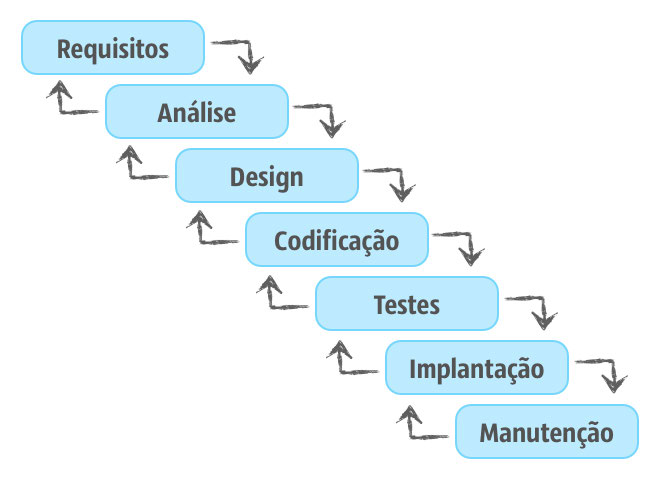
\includegraphics[scale=0.4]{imagens/CASCATA}
	\subcaption{\textbf{Fonte:} \cite{gomes2014agile}}
	\label{fig:figura1}
\end{figure*}
\FloatBarrier

Dentre as inúmeras técnicas denominadas ágeis presentes e disponíveis no mercado, pode-se destacar:

\begin{itemize}
%cap 1 pag 12 +/-
\item{\textbf{\textit{Scrum}}}: Desenvolvido em meados de 1990 por Ken Schwaber, Jeff Shuterlande Mike Beedle, o \textit{framework Scrum} está entre os mais aplicadas no mercado, com ênfase na administração de projetos, a ferramenta fomenta a acabativa\footnote{Neologismo criado por Stephen Kanitz, que segundo o autor é "a capacidade que algumas pessoas possuem de terminar aquilo que iniciaram ou concluir o que outros começaram \cite{Acabativa}."} no desenvolvimento de \textit{software} e na maioria dos casos é implementado juntamente com outras ferramentas ágeis \cite{wildt2015extreme}. 
%cap 1 pag 12 +/-
\item{\textbf{\textit{eXtreme Programming}}}: Criado por Kent Beck, Ward Cunningham e Ron Jeffries, comumente chamado de \textit{XP}, a técnica \textit{eXtreme Programming} foi idealizada para equipes intermediárias, o \textit{XP} foca principalmente na programação e nos testes. Seu propósito é a elevação do nível de confiabilidade, manutenabilidade e reusabilidade dos algoritmos desenvolvidos \cite{wildt2015extreme}.

\item{\textbf{\textit{Kanban}}}:
Na língua japonesa \textit{Kanban} quer dizer cartão sinalizador. Em contrapartida das outras técnicas ágeis, o \textit{Kanban} não impõe etapas, a ferramenta visa o aumento de produtividade por meio de uma melhor apresentação do \textit{workflow}, separando as atividades em etapas. É a metodologia ágil que menos impõe regras \cite{gomes2014agile}.
\end{itemize}

Em Scrum, XP e Kanban, há uma menor quantidade de prescrições a se seguir, facilitando a adaptação, conforme Figura 2.

\FloatBarrier
\begin{figure*}[!htbp]
	\centering
		\caption{Métodos ágeis e seus níveis de prescrição e adaptação} 
	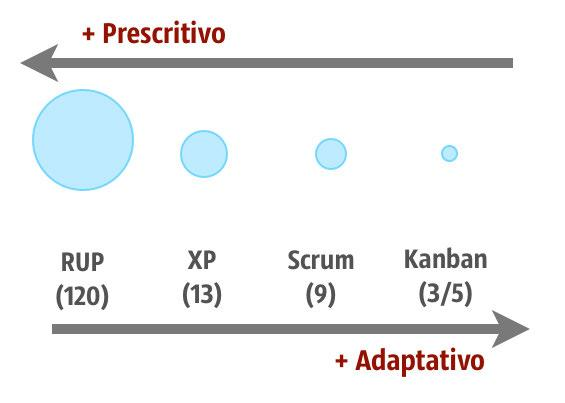
\includegraphics[scale=0.5]{imagens/prescricao}
	\subcaption{\textbf{Fonte:} \cite{gomes2014agile}} 
	\label{fig:figura2}
\end{figure*}
\FloatBarrier

\section{Tecnologias e Linguagens de Programação para Dispositivos Móveis}

Quando fala-se em aplicação móvel, na verdade referem-se aos programas que realizam operações específicas em \textit{smartphones}, \textit{tablets} e dispositivos \textit{wearables} \cite{Abranches2018}.

\subsection{Desenvolvimento Nativo para \textit{Android}}

Apesar das aplicações móveis multiplataforma ganharem mais espaço a cada ano, as aplicações mais bem-sucedidos do mercado mundial como o \textit{Facebook Messenger} e \textit{Whatsapp} foram desenvolvidos de forma nativa \cite{Abranches2018}. 

\subsubsection{Linguagem \textit{Java}}
%páginas 02 e 03%
A linguagem de programação \textit{Java} já a algum tempo é predominante na \textit{web} (\textit{World Wide Web} - WWW), a linguagem transformou a compreensão sobre desenvolvimento de sistemas, tornando-se indispensável para aqueles que almejam serem especialistas da área. Com fortes heranças de linguagens como \textit{C} e \textit{C++} e incorporando avanços e outras capacidades, \textit{Java} foi criado por James Gosling, Patrick Naughton, Chris Warth, Ed Frank e Mike Sheridan em 1991 na até então \textit{Sun Microsystems} atual \textit{Oracle Corporation}. Com o objetivo de se obter uma linguagem portátil, livre de outros programas e que fosse capaz de ser funcional nos aparelhos digitais comuns no dia-a-dia \cite{Herbert}.

%página 16 e 17
A linguagem ganhou grande repercussão em 1995 devido a sua mobilidade, possível graças a sua \textit{Java Virtual Machine} (Máquina Virtual \textit{Java} - \textbf{\textit{JVM}}) que atua como uma tradutora, transformando todo o código \textit{\textbf{bytecode} \textit{Java}} em um idioma compreendido pelo computador, independente se o sistema operacional utilizado é um \textit{Windows}, \textit{Linux} ou \textit{macOS}. Com a ausência de uma \textit{JVM}, seria necessário escrever códigos modificados para cada uma das plataformas \cite{Burd}, conforme apresentado na Figura 3.

\FloatBarrier
\begin{figure*}[!htbp]
	\centering
		\caption{Execução de um programa de computador}
	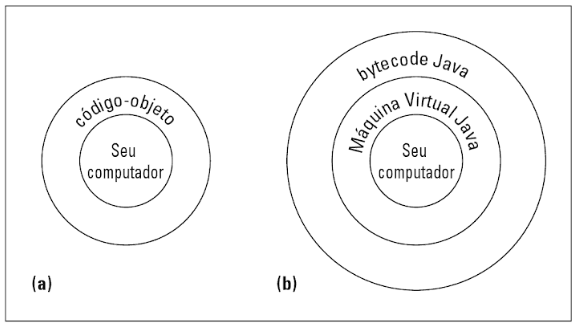
\includegraphics[scale=0.5]{imagens/JVM}
	\subcaption{\textbf{Fonte:} \citeauthorandyear{Burd}}
	\label{fig:figura3}
\end{figure*}
\FloatBarrier

\subsubsection{Plataforma \textit{Android}}

%pag 6
Criado pela \textit{Android Inc}, o sistema \textit{Android} foi comprado pela \textit{Google} em 2005, e desde 2007 vem sendo suportado pela \textit{OHA} (\textit{Open Handset Aliance}) grupo formado por gigantes da tecnologia como \textit{HTC}, \textit{Sony}, \textit{Dell}, \textit{Motorola}, \textit{Qualcomm}, \textit{Texas Instruments}, a própria \textit{Google}, \textit{Samsung}, \textit{LG}, \textit{T-mobile}, \textit{Sprint Corporation}, \textit{Nvidia}, \textit{Wind River Systems}, \textit{Asus}, \textit{Intel} e outras \cite{DeitelDeitelWald2016}.

%pag 4
Aplicativos móveis voltados para a plataforma portátil da \textit{Google}, devem ser criados com a linguagem de programação \textit{Java}, escolhida por ser uma das mais utilizadas pelos desenvolvedores, empresas e instituições de ensino e não ter nenhum custo, uma vez que é \textit{open source}\footnote{A expressão \textit{open source} de origem americana, remete a \textit{softwares} que possuem o seu código fonte aberto para contribuições. \cite{openSourceCanalTech}}  Com isso, desenvolvedores com anos, tendem a ter uma curva de aprendizado pequena em relação ao \textit{Android}, se comparado aos programadores que não possuem experiência com a linguagem \cite{DeitelDeitelWald2016}.

%pag 11
Aparelhos com o sistema operacional \textit{Android} possuem funcionalidades como acesso à internet, música, vídeo, Sistema de Posicionamento Global (\textit{Global Positioning System} - \textit{GPS}), câmera, tela sensível ao toque, dentre outras inúmeras funções. A \textit{Play Store} é a loja oficial para adicionar, avaliar, procurar e realizar o \textit{download} das aplicações disponíveis \cite{DeitelDeitel2016}.

O sistema operacional da \textit{Google} tem previsão de continuar como o mais vendido até 2022 \cite{IDC}. Conforme Tabela~\ref{tab:tabela1} e Figura 4.

\FloatBarrier
\begin{table}[!htbp]
\centering
\caption{Participação no mercado mundial de \textit{smartphones}.}
	\begin{tabular}{ c | c | c | c | c | c | c | c }
		\hline
		\textbf{Ano} & \textbf{2016} & \textbf{2017} & \textbf{2018} & \textbf{2019}  & \textbf{2020} & \textbf{2021} & \textbf{2022}  \\ \hline
		\textit{Android}      & 84,6\%        & 85,1\%        &  84,7\%       & 85,2\%         & 85,3\%        & 85,4\%        & 85,5\%  \\ \hline
		\textit{iOS}          & 14,7\%        & 14,7\%        & 15,1\%        & 14,8\%         &14,6\%         & 14,6\%        & 14,5\%     \\ \hline
		Outros       & 0,7\%         & 0,2\%         & 0,1\%         & 0,1\%          & 0,1\%         & 0,1\%         & 0,1\% \\ \hline
	\end{tabular}
	\\ \vspace{0.2cm}
		\subcaption{\textbf{Fonte:} Adaptado pelo autor - \cite{IDC}}
	\label{tab:tabela1}
\end{table}
\FloatBarrier

\FloatBarrier
\begin{figure*}[!htbp]
	\centering
		\caption{Gráfico de participação no mercado mundial de \textit{smartphones}.}
	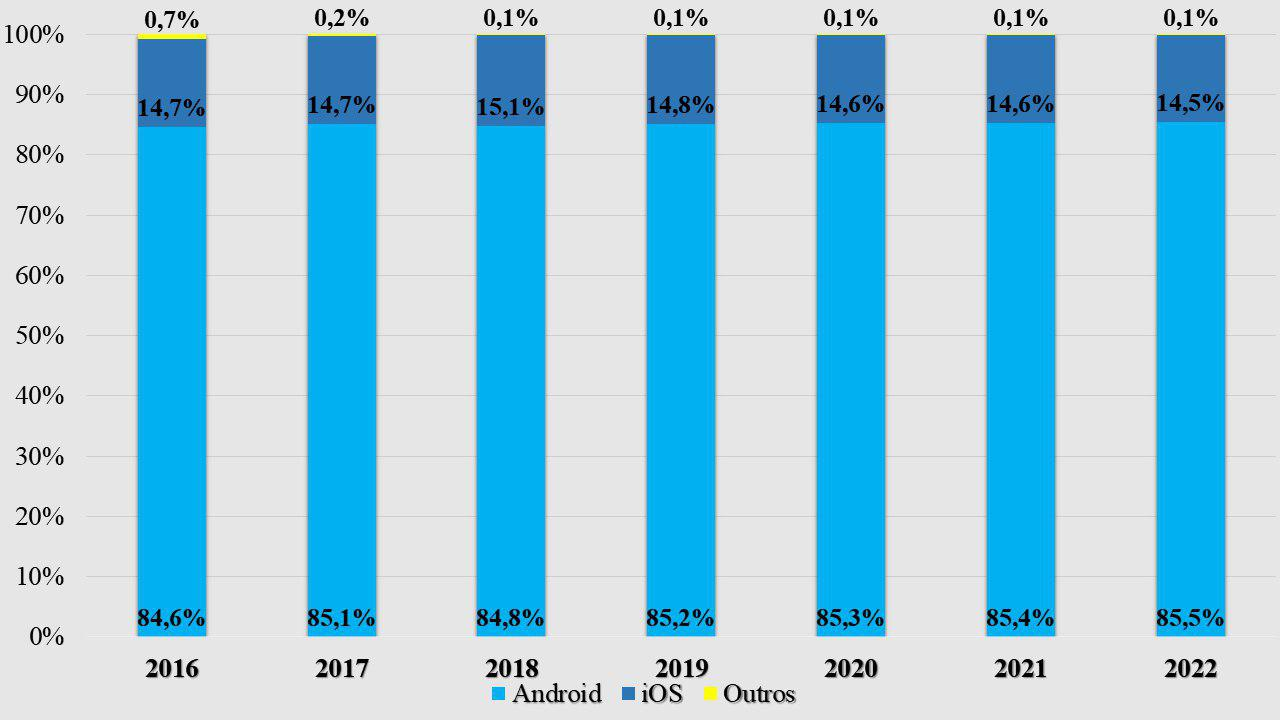
\includegraphics[scale=0.4]{imagens/IDC}
	\subcaption{\textbf{Fonte:} Adaptado pelo autor - \cite{IDC}}
	\label{fig:figura4}
\end{figure*}
\FloatBarrier

\subsection{Desenvolvimento Nativo para \textit{iOS}}

%pag 23
Tanto os usuários como os desenvolvedores que buscam por um \textit{design} mais sofisticado, uma riqueza maior em detalhes, aliados a uma comunicação diferenciada com o aparelho móvel, encontram como opção o \textit{iPhone}, que possui \textit{iOS}, o sistema operacional móvel da empresa americana \textit{Apple Inc.}, o mais utilizado após o \textit{Android} \cite{Lecheta2016_IOS_&_IPAD}.

%pags 23 e 24
Anunciado em 2007 em uma conferência voltada para programadores, no mesmo ano o \textit{smartphone iPhone} conseguiu ganhar seu lugar de destaque entre os usuários comuns e do mundo da tecnologia, devido a capacidade e qualidade dos recursos presentes no pequeno aparelho móvel, obteve também a atenção dos programadores, uma vez que sua loja oficial, a \textit{Apple Store} prometia uma gratificação, o que até o momento era novidade \cite{Lecheta2016_IOS_&_IPAD}.

%pags 2
Apesar de lançado em 2007, somente no ano seguinte tornou-se possível programar voltado para o \textit{iOS}, por meio do Kit de Desenvolvimento de \textit{Software} (\textit{Software Development Kit - SDK}), porém o \textit{SDK} passou a ser gratuito apenas três anos mais tarde. Para utilizar-se o \textit{iOS SDK}, é obrigatório possuir um computador com no mínimo o sistema operacional \textit{macOS X} instalado, caso contrário, não será possível nem mesmo realizar o \textit{download}. Recentemente, o \textit{SDK }passou a ser disponibilizado com o ambiente integrado oficial de desenvolvimento para a plataforma \textit{iOS}, o \textit{Xcode IDE} \cite{Steil_IOS}.

%pags 187 
\subsubsection{Linguagem \textit{Objective-C}}
Adquirida e licenciada em 1988 pela empresa \textit{Apple Inc.}, a linguagem 
\textit{Objective-C} foi fundamental no desenvolvimento de aplicações voltadas para \textit{iOS} e \textit{macOS}. Pode-se dizer que apesar da diferença na escrita de algoritmos, \textit{Objective-C} é na verdade \textit{C} com o acréscimo de várias funcionalidades como o paradigma de programação, portanto \textit{Objective-C} é totalmente interoperável com tudo que já existe e que foi escrito originalmente utilizando-se a linguagem \textit{C} \cite{Steil_IOS}.  

Dado ao avanço das linguagens de programação e das tecnologias envolvidas, o \textit{Objective-C} acabou tornando-se um tanto quanto obsoleto quando comparado a outras linguagens mais sucintas e com curva de aprendizado consideravelmente inferiores. Para mudar esse cenário, e fazer com o que a programação voltada para seus produtos voltasse a ser atrativa, a \textit{Apple} lançou a linguagem \textit{Swift} \cite{SwiftINFOQ2015}.

\subsubsection{Linguagem \textit{Swift}}
%Impressionante o que estãofazendo com Swift.
Com uma grande influência de linguagens mais modernas como \textit{Scala} e \newcommand{\Csh}{\textit{C}{\lserif\#}}\Csh{}, \textit{Swift} foi desenvolvida para ser fácil e compatível com mais de um paradigma de desenvolvimento \cite{SwiftINFOQ2015}. É voltada para os principais produtos da \textit{Apple}, como \textit{iOS}, \textit{macOS}, \textit{Apple Tv} e \textit{Apple Watch}, possui total compatibilidade com algoritmos legados escritos em \textit{Objective-C}. Aplicações feitas em \textit{Swift} são menos vulneráveis e poupam consideravelmente tempo em seu desenvolvimento \cite{SwiftAPPLE2019}.

%O código Swift está aberto para todos.
Grande parte, senão a maioria dos programadores com foco em produtos \textit{Apple} migraram de \textit{Objective-C} para \textit{Swift} e já constroem aplicações usando somente a nova linguagem no \textit{backend}. Aplicações \textit{Swift} chegam a ser \textbf{2,6} vezes mais velozes do que aplicações em \textit{Objective-C} e \textbf{8,4} vezes mais ágeis em comparação com \textit{Python} na sua versão 2.7. Por ser uma linguagem \textit{open source}, ganhou espaço tanto no meio educacional como profissional \cite{SwiftAPPLE2019}. 

\subsection{Desenvolvimento Multiplataforma}

% 1º PAGINA DA INTRODUÇÃO CAP 1
Com todo o avanço das tecnologias envolvidas nos dispositivos móveis, a \textit{Google} tinha seu próprio sistema, assim como \textit{Apple}, \textit{Microsoft}, \textit{BlackBerry} e outros que com o passar dos anos acabaram sendo descontinuados, ou ficaram com uma fatia quase inexistente no mercado. Porém cada empresa seguiu por caminhos diferentes como: \textit{frameworks}, linguagens e máquinas virtuais, o que acabou culminando na incompatibilidade das plataformas, fazendo-se necessário a criação de aplicações específicas para cada público \cite{IONIC2017_ADRIAN_GOIS}.

\subsubsection{\textit{Xamarin Framework}}

%1.2 ...
Utilizando-se todo o potencial e funcionalidades da linguagem \newcommand{\Csh}{\textit{C}{\lserif\#}}\Csh{} da empresa americana Microsoft, tornou-se possível construir aplicações móveis tanto para a plataforma \textit{iOS}, \textit{Android} e para a recentemente descontinuada \textit{Windows Phone} e até mesmo para o sistema operacional \textit{Windows}. Anteriormente fazia-se necessário pagar pela utilização da ferramenta \textit{Xamarin}, o que acabou mudando após sua venda para a \textit{Microsoft}. Atualmente, é uma ferramenta sem custo e de código \textit{open source} \cite{XAMARIN2017}.
%1.3
Pode-se aproveitar entre 75\% a 100\% de qualquer algoritmo já existente para utilização em desenvolvimento para qualquer um dos ambientes suportados, fazendo-se necessárias pouquíssimas alterações para chegar ao objetivo desejado de programação multiplataforma, alcançando-se assim o total aproveitamento do sistema utilizado, da linguagem \newcommand{\Csh}{\textit{C}{\lserif\#}}\Csh{} e da plataforma \textit{.NET}, já na parte de Interface e Experiência do Usuário (\textit{User Experience} e \textit{User Interface} - \textit{UX/UI}) utiliza-se o \textit{Xamarin Forms}, onde aplica-se \newcommand{\Csh}{\textit{C}{\lserif\#}}\Csh{} e/ou \textit{XAMAL}, aproveita-se totalmente uma tela em qualquer ambiente suportado pelo \textit{Xamarin} sem nenhuma complicação ou ajuste manual a ser realizado pelo desenvolvedor \cite{XAMARIN2017}.

\subsubsection{\textit{IONIC Framework}}
% Acho que pagina do cap1 introducao
O \textit{framework PhoneGap/Cordova} trouxe com ele esperança para empresas e desenvolvedores do ramo da programação conseguirem evitar o \textbf{retrabalho} de criação de aplicações móveis específicas para cada fatia do mercado, por meio do aproveitamento dos já consolidados \textit{HTML}, \textit{CSS} e \textit{JavaScript} para criação de uma categoria intermediária. O \textit{IONIC Framework} criado em 2013, apoia-se em ferramentas focadas no \textit{front-end} como \textit{PhoneGap/Cordova} juntamente com o \textit{AngularJS} e outros recursos para criação de aplicações multiplataforma \cite{IONIC2017_ADRIAN_GOIS}, conforme apresentado na Figura 5. 

\FloatBarrier
\begin{figure*}[!htbp]
	\centering
		\caption{Fluxo de conversão do \textit{PhoneGap}}
	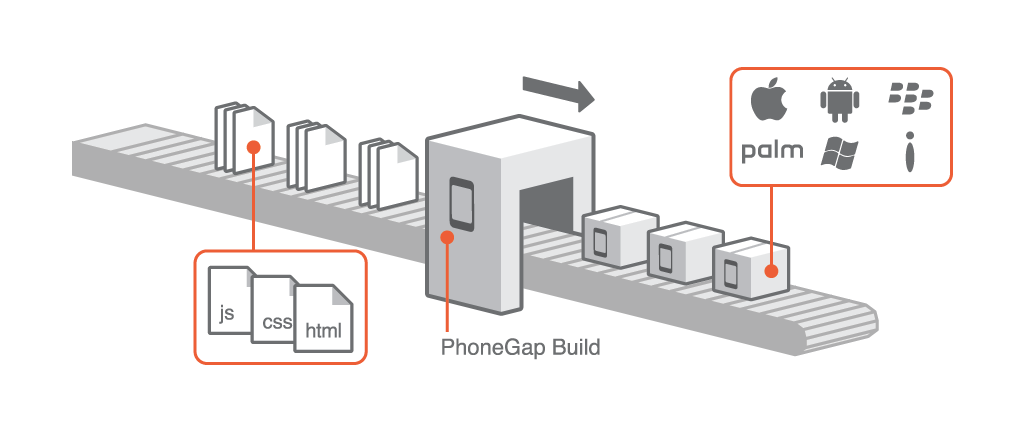
\includegraphics[scale=0.4]{imagens/PHONEGAP}
	\subcaption{\textbf{Fonte:} \citeauthorandyear{IONIC2017_ADRIAN_GOIS}}
	\label{fig:figura3}
\end{figure*}
\FloatBarrier

A programação com base em \textit{PhoneGap/Cordova} por meio de tecnologias de \textit{front-end}, torna possível a concepção (\textbf{\textit{build}}) de aplicações móveis nativas para as plataformas \textbf{alvo}, esses aplicativos desempenham características semelhantes aos programas nativos, pois o \textit{software} está sendo compilado incorporado em uma  espécie de navegador de internet, denominado de \textit{webview}, porém, essa abstração com o navegador \textit{webview} é invisível e imperceptível para os seus utilizadores. Esse navegador adaptado beneficia-se primordialmente da linguagem de marcação \textit{HTML}, de uma folha de formatação de estilo \textit{CSS} e do \textit{JavaScript} para sua exibição e funcionamento \cite{IonicCordovaMedium2017}. Para criar-se uma aplicação compatível com mais de um sistema operacional com o \textit{IONIC Framework}, faz-se necessária a instalação do \textit{IONIC Framework CLI}, \textit{JDK} versão 7, \textit{SDK do Android}, \textit{NodeJS} e um editor de texto ou \textit{IDE} compatível \cite{IONIC2017_ADRIAN_GOIS}.

\subsection{Linguagem \textit{Kotlin}}
%pagi dona 38
Em 2017, foi divulgado que seria possível desenvolver aplicações móveis nativas voltadas para o sistema operacional \textit{Android} utilizando não somente a linguagem \textit{Java}, mas também desenvolver com \textit{Kotlin}, todo o público presente no evento \textit{Google I/O} apoiou e aprovou o pronunciamento. Com tal possibilidade de se escolher entre as duas linguagens e até mesmo mesclá-las nos mesmos projetos, classes e afins, o desenvolvimento \textit{Android} tornou-se muito mais proveitoso \cite{Lecheta2018}.

A motivação para criação do Kotlin foi basicamente suprir as necessidades encontradas pela equipe da JetBrains durante os anos de desenvolvimento de ambientes integrados como \textit{IntelliJ}, \textit{PyCharm}, \textit{RubyMine} e \textit{WebStorm} usando \textit{Java} como linguagem principal e também \textit{Scala}. A linguagem foi batizada com o nome da ilha Russa de \textit{Kotlin} localizada próxima a São Petersburgo \cite{Lecheta2018}.

%pagina 38
Tanto \textit{Kotlin} como o  \textit{Android Studio} que é a  \textit{IDE} oficial de desenvolvimento  \textit{Android}, foram criados pela empresa russa  \textit{JetBrains}. Sua sintaxe de fácil compreensão proporciona uma programação mais prazerosa. Possui total compatibilidade com a linguagem \textit{Java} pois ambas utilizam a \textit{JVM} \cite{Lecheta2018}.

% cap 1.1
A linguagem começou a ser desenvolvida em 2011, com base no vasto conhecimento da empresa \textit{JetBrains} no desenvolvimento e suporte de \textit{IDE's} tanto para \textit{Java} como para vários outros tipos de tecnologias, com a intenção de chegar-se a uma linguagem que poderia ser executada e/ou usada nos mesmos projetos onde \textit{Java} era utilizado e não somente para o ecossistema \textit{Android}\footnote[4]{O ecossistema Android é composto pelas linguagens suportadas pela \textit{JVM} referente a programação Android nativa, ambiente (\textit{IDE}) e kit de desenvolvimento e a loja oficial na qual os aplicativos são disponibilizados \cite{EcossitemaAndroid}}. Em meados de 2006, já havia a possibilidade de se realizar o \textit{download} do complemento e instalar na \textit{IDE Android Studio} para programar em \textit{Kotlin} para \textit{Android} \cite{Resende2018}. 

A seguir os pontos que tornam a linguagem tão relevante no mercado de desenvolvimento \cite{Resende2018}:

\begin{itemize}
% cap 1.4
\item \textbf{Sucinta:} A característica de ser uma linguagem com sintaxe bem sucinta em relação ao \textit{Java}, significa que ao converter um arquivo/classe \textit{Java} para \textit{Kotlin} o resultado final será o mesmo, porém em uma abordagem com \textit{Kotlin} teria-se menos códigos desnecessários, como uma classe sem métodos acessores e modificadores explícitos por exemplo, o que facilita em muito a leitura e manutenção de código, essa conversão pode ser realizada tanto de forma manual ou com recursos da própria \textit{IDE Android Studio}. %\cite{Resende2018}.

% cap 1.5 ??
\item \textbf{Protegida contra exceções:} Uma das exceções mais encontradas na programação \textit{Java}, com certeza é \textit{NullPointerException} que se trata de uma menção a algo que ainda não está disponível a nível  de programa. Em \textit{Kotlin} \textbf{não} é possível atribuir o valor nulo a uma variável, para forçar uma variável a receber um valor nulo é necessário adicionar um \textbf{ponto de interrogação} na declaração do tipo. %\cite{Resende2018}. 

\item \textbf{Desejada:} 2º linguagem de desenvolvimento mais querida, a 4º mais pesquisada e a 22º mais admirada do ano de 2018, segundo pesquisa realizada com mais de 100 mil usuários de todas as partes do mundo. %\cite{StackOverFlow2018}.

\item \textbf{Integrada:} Desde a versão 3.0 da \textit{IDE Android Studio}, fez-se desnecessária a instalação de \textit{plugins Kotlin}, pois o complemento passou a ser disponibilizado totalmente integrado com o ambiente de desenvolvimento.% \cite{Teodosio}.

% cap 1.3
\item \textbf{Compatível\footnote{ \textit{\textbf{ART} Android Runtime}: Ambiente de tempo de execução a partir do \textit{Android} 5 e superior.
\textit{\textbf{DALVIK} Android Runtime}: Ambiente de tempo de execução em versões inferiores ao \textit{Android} 5. \cite{ArtDalvik}}:} A total compatibilidade entre a linguagem da empresa \textit{JetBrains} e \textit{Java}, permite a troca de dados entre arquivos tanto na extensão .kt como .java. %\cite{Resende2018}. 
\end{itemize}

Os arquivos que possuem extensão .kt foram desenhados e idealizados desde sua concepção para possibilitarem sem maiores dilemas e complicações inúteis as chamadas aos arquivos de extensão .java de forma totalmente nativa e eficaz, conforme apresentado na Figura 6. %\cite{JetbrainsDocs}

\FloatBarrier
\begin{figure*}[!htbp]
	\centering
		\caption{Fluxo de conversão de códigos Kotlin e Java para \textit{bytecode}} 
	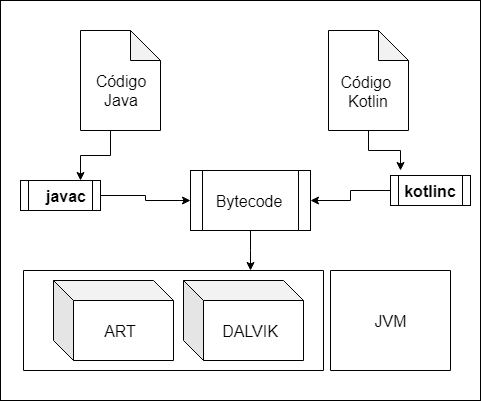
\includegraphics[scale=0.5]{imagens/androidKotlinJVM}
\subcaption{\textbf{Fonte:} Adaptado pelo autor} - \cite{SlideShare}
	\label{fig:figura4}
\end{figure*}
\FloatBarrier


\section{Qualidade de Código}
Qualquer profissional da área de tecnologia e programação tem plena de consciência da qualidade dos seus códigos, porém, em projetos consideravelmente maiores, e com muitos responsáveis, pode ocorrer a perda da qualidade no projeto. Para sanar essas adversidades, existem diversos programas, que realizam de forma automática ou não, o controle e a análise de qualidade, produzindo relatórios técnicos, entretanto, nem sempre se chega ao resultado esperado \cite{qualidadedesoftware}. 

\subsection{Refatoração de Código}
A técnica de refatoração propõe examinar os códigos já existentes, com o objetivo de se reduzir repetições (desnecessárias) e incoerências presentes no sistema \cite{lindstrom2017refatoracao}. Com a falta da prática de se refatorar, os projetos acabam tornando-se muito complexos, inviabilizando futuras alterações e correções, chegando ao ponto de se cogitar a total reescrita de um sistema, independente do seu tamanho e importância. Em seu livro Código Limpo, o renomado autor Robert C. Martin definiu alguns parâmetros para uma refatoração eficiente \cite{ZanetteBeCodeCleanCode2017}: 

\begin{itemize}
\item{\textbf{Nomenclaturas}}:
Deve-se declarar operações, propriedades, parâmetros e classes de forma condizente com sua função, para que  ao realizar a leitura, seja fácil identificar o seu verdadeiro propósito. As nomenclaturas devem ser as mais fiéis possíveis, mesmo que para se alcançar o objetivo, seja necessária uma nomenclatura relativamente grande. Operações necessitam obrigatoriamente serem declaradas com nomenclatura de verbos, e classes e suas instâncias necessitam estar declaradas como substantivos \cite{ZanetteBeCodeCleanCode2017}.

\item{\textbf{Operações}}:
Robert C. Martin, diz que as operações devem ser curtas e descomplicadas, o quanto menor for uma operação, melhor. Uma operação só pode executar exclusivamente uma atividade, isso vai oportunizar o reaproveitamento da operação, dessa forma será mais fácil a revisão e conservação do código \cite{ZanetteBeCodeCleanCode2017}.

\item{\textbf{Comentários/Anotações}}:
Deve-se comentar o mínimo possível, pois apesar dos sistemas estarem sempre em modificações, os comentários acabam sendo esquecidos e pode vir a prejudicar futuramente. Portanto ao utilizá-lo, deve ser sempre revisado \cite{ZanetteBeCodeCleanCode2017}.

\item{\textbf{Duplicidades}}:
Cada parte de compreensão do código, necessita ser exclusiva, pois é prejudicial trechos semelhantes de código que executam a mesma operação em lugares diferentes, pois torna-se muito mais difícil e passível de esquecimento realizar uma mesma modificação em múltiplos locais dentro de um programa. Mesmo que nem toda duplicidade afete razoavelmente, aconselha-se livrar-se delas \cite{ZanetteBeCodeCleanCode2017}.

\item{\textbf{Prevenção}}:
Deve-se aproveitar ao máximo os recursos de tratamentos e exceções e erros, oferecidos pela maioria das linguagens de programação disponíveis, tomando \textit{Java} como exemplo, temos disponíveis \textit{Exceptions} e blocos \textit{try-catch}. Um sistema necessita estar pronto para as situações adversas das idealizadas por seu criador. Orienta-se também, evitar os valores nulos em qualquer parte, sempre que possível \cite{ZanetteBeCodeCleanCode2017}.

\item{\textbf{Reescrita}}:
Deve-se criar a rotina de reescrita de código, com isso o sistema estará sempre atual, o ideal é reescrever enquanto a raciocínio utilizado ainda está recente na mente do desenvolvedor, mas deve-se tentar evitar sempre a criação de possíveis novos \textit{bugs} \cite{ZanetteBeCodeCleanCode2017}. 

\item{\textbf{Verificação}}:
Os testes de \textit{software} necessitam ser eficazes, ágeis, individuais, sem duplicidades e efetuar sempre a operação que para a qual foi-se desenhado e programado para realizar. Orienta-se a aplicação do \textit{TDD}, ou seja, primeiro criando a operação de testes, em seguida o trecho de código a ser verificado e após a conclusão, deve-se refatorar \cite{ZanetteBeCodeCleanCode2017}.

\end{itemize}

\subsection{Ferramentas para Análise de Qualidade de Código}

Entende-se por Analisadores Estáticos de Códigos (AEC), os programas capazes de identificar, enumerar e até mesmo solucionar imperfeições e falhas existentes em um \textit{software}, o que possibilita que desenvolvedores e gerentes de projeto preocupem-se com outros fatores de um sistema, uma vez que se tem uma ferramenta específica para realização de uma análise mais detalhada \cite{AECMedium2018}. 

Com a utilização de um AEC, as falhas e possíveis ameaças são prontamente detectadas, e isso é realizado dentre outras funcionalidades pela análise de:

\begin{itemize}
    \item \textbf{Quantidade de linhas de código} (\textit{Lines of code} - \textit{LOC}) utilizadas, o que pode variar de acordo com as linguagens de programação (mais ou menos verbosas) empregadas no projeto \cite{DevQA}.
    
    \item {\textbf{Quantidade de instruções condicionais e de repetição} (\textit{Cyclomatic Complexity} - \textit{CC}) aconselha-se que esse número seja sempre o mais baixo possível segundo Robert C. Martin, autor do livro \textit{Clean Code}. \cite{DevQA}.}
    
    \item{\textbf{Coerência das operações} (\textit{Lack of Cohesion of Methods} - \textit{LCOM}) no qual são quantificadas as responsabilidades exercidas pelo conteúdo de uma classe. \cite{DevQA}.}
\end{itemize}

\subsubsection{\textit{SonarQube}}
Anteriormente chamado apenas de \textit{Sonar}, o \textit{SonarQube} desenvolvido pela \textit{SonarSource SA}, é um sistema \textit{web} de código fonte aberto que realiza a verificação das características de um programa e exibe os resultados obtidos por meio de um painel \cite{AECMedium2018}, conforme Figura 7. Dentre suas muitas possibilidades de análise, destacam-se as verificações de padrões de projeto, duplicidade de código e prevenção contra as possíveis inconsistências \cite{DevQA}.

Além de ser personalizável ao gosto do usuário, o programa oferece ainda a possibilidade de ser utilizado juntamente com diversos ambientes de desenvolvimento integrado disponíveis no mercado e também com sistemas de versionamento de projeto como o \textit{GitHub} da \textit{Microsoft}, possibilitando uma oportunidade para efetuar-se correções e ajustes de problemas antecedendo futuras alterações e problemas relacionados ao versionamento \cite{DevQA}. 

\FloatBarrier
\begin{figure*}[!htbp]
	\centering
		\caption{Parte do Painel do \textit{SonarQube}} 
	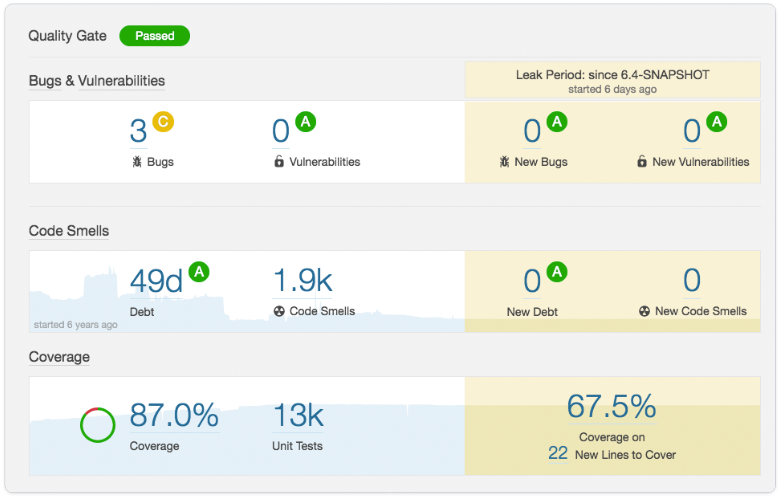
\includegraphics[scale=0.6]{imagens/SONAR2}
  \subcaption{\textbf{Fonte:} \cite{SonarSite}}
	\label{fig:figura7}
\end{figure*}
\FloatBarrier

\subsubsection{\textit{Ebert}}

 O \textit{Ebert} é um sistema pago e desenvolvido pela \textit{Caliper Metrics} parte da empresa brasileira Plataformatec que provê uma análise tanto estática como contínua dos códigos desempenhados, por meio de uma total integração com o sistema versionamento de projetos \textit{GitHub}, com a sua utilização a equipe torna-se muito mais apta para visualizar os erros, recebendo sugestões para solução e também dicas para desviar-se deles pelo decorrer de todo o projeto. O sistema abstrai dos envolvidos a necessidade de uma verificação de alterações de códigos submetidos para entrar em produção, notificando instantaneamente sobre brechas de segurança, duplicidades, incoerências desnecessárias, incompatibilidades e também permite vários ajustes e modificações referentes às verificações de código apresentadas, conforme apresentado na Figura 8 \cite{Ebert}.
 
 \FloatBarrier
\begin{figure*}[!htbp]
	\centering
		\caption{Interface do \textit{Ebert}} 
	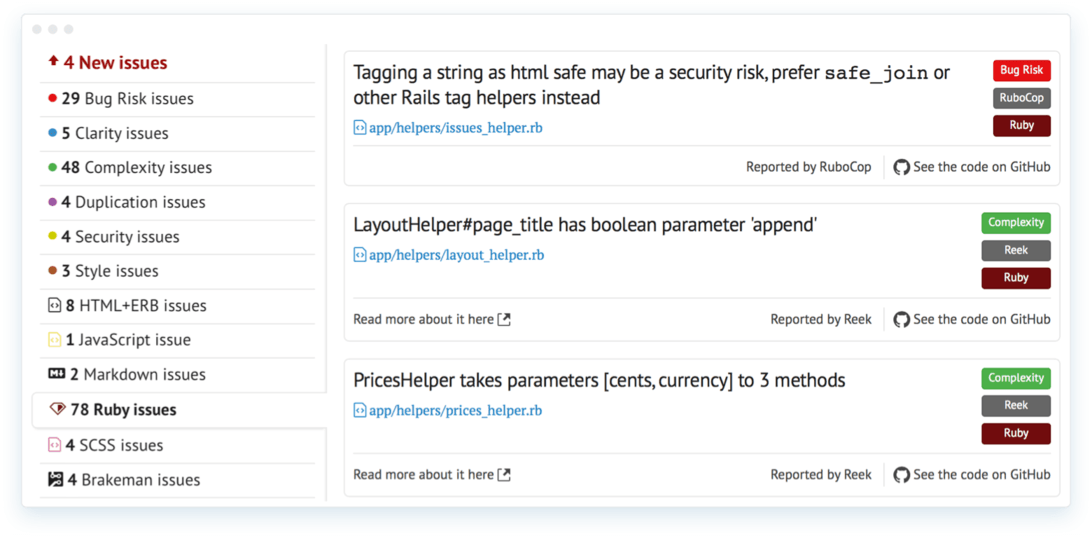
\includegraphics[scale=0.4]{imagens/Ebert}
  \subcaption{\textbf{Fonte:} \cite{Ebert}}
	\label{fig:figura7}
\end{figure*}
\FloatBarrier

\section{Trabalhos Relacionados a esta Pesquisa}

Nesta subsecção, serão apresentados alguns trabalhos relacionados ao tema principal da pesquisa: a linguagem de programação \textit{Kotlin} e a qualidade de \textit{software} por meio de técnicas e tecnologias.

\subsection{Desenvolvimento de Aplicativo para Adoção de Animais Abandonados Utilizando a Linguagem de Programação \textit{Kotlin} e Programação Reativa \cite{TccKotlin}}

O intuito do trabalho realizado na Universidade Tecnológica Federal do Paraná nos Departamentos de Acadêmicos de Eletrônica e Informática no curso Engenharia da Computação é de se minimizar o número de animais desabrigados nas grandes cidades como Curitiba, com a criação de uma aplicação móvel nativa, destinada para usuários do sistema operacional \textit{Android}, utilizando os recursos oferecidos pela linguagem de programação \textit{Kotlin} para obter-se mais uma opção para auxiliar as ferramentas já existentes destinadas a facilitar o encontro e a adoção dos animais de rua \cite{TccKotlin}.

Apesar das dificuldades em utilizar algumas tecnologias de armazenamento de dados mais atuais como o \textit{Firebase}, as metas desejadas foram alcançadas com a criação de uma aplicação móvel em uma linguagem de desenvolvimento ainda pouco conhecido para os meios acadêmicos mas que ofereceu inúmeros aspectos que facilitaram em muito a programação, o projeto encabeçou aumentar a integração das \textit{ONG's} com os interessados em adoção. Como ideia para próximos passos ficaram a criação de um sistema destinado para usuários do sistema operacional \textit{iOS} e a resolução de alguns \textit{bugs} simples, mas que facilitaram a usabilidade do sistema. No decorrer do desenvolvimento da pesquisa, \textit{Kotlin} passou a ser a nova linguagem de desenvolvimento oficial para \textit{Android} \cite{TccKotlin}. 

\subsection{\textit{Framework} para Avaliação da Qualidade de Código: Uma
Abordagem Baseada em Valor \cite{Framework}}
A meta da pesquisa realizada na Universidade de Brasília, era a análise e o acompanhamento de algumas metodologias denominadas ágeis, juntamente com técnicas de testes de unidade de \textit{software} para obtenção de sistemas menos propensos a futuro/possíveis erros provenientes da falta de averiguação por parte dos envolvidos \cite{Framework}. 

Com o cumprimento da meta geral e das específicas como primeira etapa do trabalho, nessa fase inicial da pesquisa, foram planejados todos os possíveis passos para aplicação e utilização do \textit{framework ágil} \textit{Scrum} e/ou \textit{XP} e dos testes de unidade, com intuito de resultar em melhores acabativas nos projetos desempenhados pela  Controladoria Geral do Distrito Federal e do Laboratório Fábrica de \textit{Software} - Campus UnB Gama, ambos localizados em Brasília. Nas etapas futuras, planeja-se colocar em prática os conceitos idealizados \cite{Framework}.

\subsection{Proposta de Plano de Garantia da Qualidade de \textit{Software} para o Laboratório de
Criação e Aplicação de \textit{Software} \cite{PropostaDePlano}}

Neste artigo desenvolvido na Universidade de Caxias do Sul - Centro de Computação e Tecnologia da Informação, tinha-se como objetivo para a pesquisa, analisar as atuais técnicas de programação empregadas no Laboratório de Criação e Aplicação de \textit{Software} da instituição, para que através dessa futura análise torna-se possível implementar pelo menos parte das ferramentas e técnicas corretas com o propósito de garantir que todos os programas desenvolvidos obtivessem maior qualidade em suas entregas, tanto para os programadores, quanto para os responsáveis técnicos pelos projetos e principalmente para os utilizadores finais. \cite{PropostaDePlano}.

Os propósitos da pesquisa foram cumpridos, mediante acompanhamento e implantação de ferramentas abertas para gerir o processo de desenvolvimento por parte dos programadores, evidenciou-se que é praticamente impossível realizar um desenvolvimento sem imperfeições e defeitos. Para trabalhos futuros, indicou-se a elaboração de uma inspeção para maiores reconhecimentos dos ganhos obtidos \cite{PropostaDePlano}.

\subsection{Estimando Atributos de Qualidade de \textit{Software}
Utilizados e Desejados pelas Empresas
Certificadas no \textit{MPS-SW} no Brasil \cite{EstimandoAtributos}}

Nesta pesquisa desenvolvida na Universidade Federal de Ouro Preto, Departamento de Computação e Sistemas, Colegiado de Engenharia de Computação, o intuito era de se elaborar uma equiparação entre a característica dos programas e sistemas entregues e características almejadas pelas empresas participantes do estudo \cite{EstimandoAtributos}.

Alcançou-se o objetivo do trabalho, mesmo com da falta de comprometimento das empresas solicitadas em se envolverem e responderem algumas perguntas e questionários simples. Constatou-se que as empresas na sua maioria, contam com metodologias ágeis no seu dia-a-dia de programação e mais instrumentos automáticos que por sua vez, executam a geração e o acompanhamento de métricas referentes às tarefas desempenhadas, principalmente os códigos desenvolvidos. \cite{EstimandoAtributos}.
